% (c) 2014 Daniele Masini - d.masini.it@gmail.com
\section{Esercizi}

\subsection{Esercizi riepilogativi}

\subsubsection*{\thechapter.1 - La misura}

\begin{esercizio}
\label{ese:6.1}
Vero o falso?
\begin{enumeratea}
\item Date due grandezze $A$ e $B$ è sempre possibile stabilire qual è la più grande\hfill\boxV\quad\boxF
\item Due grandezze geometriche si dicono commensurabili quando esiste una terza grandezza che è sottomultipla comune alle altre due \tab\hfill{\boxV\quad\boxF}
\item Un qualunque numero razionale può essere definito come elemento separatore di due classi numeriche contigue\hfill\boxV\quad\boxF
\item La misura di un segmento è un segmento\hfill\boxV\quad\boxF
\item la diagonale di un quadrato è incommensurabile con il lato\hfill\boxV\quad\boxF
\end{enumeratea}
\end{esercizio}

\begin{esercizio}
\label{ese:6.2}
L'insieme delle ampiezze degli angoli rappresenta una classe di grandezze omogenee? Giustifica la risposta.
\end{esercizio}

\begin{esercizio}
\label{ese:6.3}
Disegna un segmento $AB$ a piacere, costruisci poi il segmento $CD=\frac{3}{5}AB$.
\end{esercizio}

\begin{esercizio}
\label{ese:6.4}
Qual è il rapporto tra i segmenti $AB$ e $CD$ rappresentati in figura~\ref{fig:ese6.4}? Indica nel disegno quale può essere l'unità di misura comune ad entrambi.
\end{esercizio}

\begin{figure}[!htb]
	\centering% Copyright (c) 2015 Daniele Masini - d.masini.it@gmail.com

\begin{tikzpicture}[scale=0.6,font=\small]
\usetikzlibrary{calc}

\begin{scope}

\begin{scope}[rotate=20]
\foreach \x in {0,1,2,3}
{
	\draw (\x, -.05) -- (\x, .05);
}
\draw (0,0) -- (3,0);
\end{scope}

\foreach \x in {0,1,2,3,4,5}
{
	\draw (\x, -1.05) -- (\x, -.95);
}
\draw (0,-1) -- (5,-1);

\end{scope}


\end{tikzpicture}

	\caption{Esercizio~\ref{ese:6.4}}\label{fig:ese6.4}
\end{figure}

\begin{esercizio}
\label{ese:6.5}
Disegna due segmenti $AB$ e $CD$ per i quali valga il rapporto $\frac{3}{2}AB=\frac{2}{3}CD$.
\end{esercizio}

\begin{esercizio}
\label{ese:6.6}
\`E possibile che due angoli siano tra loro incommensurabili?
\end{esercizio}

\begin{esercizio}
\label{ese:6.7}
\`E possibile che i perimetri di due quadrati siano tra loro incommensurabili? Fai un esempio.
\end{esercizio}

\begin{esercizio}
\label{ese:6.8}
In quali casi le due grandezze $A$ e $B$ sono incommensurabili?
\begin{multicols}{4}
\begin{enumeratea}
\item $A=\frac{1}{3}B$;
\item $A=\np{1,3}B$;
\item $A=\np{1,}\overline{3}B$;
\item $A=\sqrt{2}B$;
\end{enumeratea}
\end{multicols}
\end{esercizio}

\begin{esercizio}
\label{ese:6.9}
Nel triangolo rettangolo $ABC$, i cateti $AB$ e $AC$ hanno rapporto $\frac{3}{4}$. Qual è il rapporto tra  l'ipotenusa $BC$ e il cateto $AB$? Sono grandezze tra di loro commensurabili?
\end{esercizio}

\begin{esercizio}
\label{ese:6.10}
Date le relazioni $AB=CD+\frac{1}{2}EF$ e $\frac{2}{3}CD=\frac{1}{4}EF$, disegna i segmenti $AB$, $CD$ ed $EF$ scegliendo un'opportuna unità di misura e determina la misura di $AB$ rispetto a $CD$. $[AB=\frac{7}{3}CD]$
\end{esercizio}

\begin{esercizio}
\label{ese:6.11}
Il segmento $AB$ misura $3a$, quanto misura rispetto a $\frac{1}{2}a$? 
\end{esercizio}

\begin{esercizio}
\label{ese:6.12}
Per quali dei seguenti valori di $a$ il numero $\sqrt{a}$ è un numero irrazionale?
\begin{multicols}{5}
\begin{enumeratea}
\item 1;
\item 2;
\item 3;
\item 4;
\item 5;
\item 6;
\item 8;
\item 9;
\item 10.
\end{enumeratea}
\end{multicols}
\end{esercizio}

\subsubsection*{\thechapter.2 - Proporzionalità tra grandezze}

\begin{multicols}{2}

\begin{esercizio}
\label{ese:6.13}
Se tra quattro grandezze omogenee è vera la proporzione $x : y = v : z$, quali delle seguenti proporzioni sono vere di conseguenza?
\begin{enumeratea}
\item $x : v = y : z$
\item $x : z = v : y$
\item $v : x = x : y$
\item $z : y = v : x$
\end{enumeratea}
\end{esercizio}

\begin{esercizio}
\label{ese:6.14}
Sapendo che $\dfrac{x}{y}=\dfrac{5}{7}$ e $\dfrac{x}{z}=\dfrac{5}{4}$ completa la proporzione $x : z = \ldots{} : \ldots{}$
\end{esercizio}

\begin{esercizio}
\label{ese:6.15}
Sapendo che $\dfrac{x}{y}=\sqrt{2}$ e $\dfrac{x}{z}=\sqrt{3}$ completa la proporzione $x : z = \ldots{} : \ldots{}$
\end{esercizio}

\begin{esercizio}
\label{ese:6.16}
Quattro grandezze $A$, $B$, $C$ e $D$ sono tali che $3A=2B$ e $3C=2D$. Verifica se sono in proporzione e in caso affermativo scrivila.
\end{esercizio}

\begin{esercizio}
\label{ese:6.17}
Dimostra che se vale la proporzione $3A : 2B = 3C : 2D$ vale anche la proporzione $A : B = C : D$.
\end{esercizio}

\begin{esercizio}
\label{ese:6.18}
Siano $A$, $B$, $C$, $D$, $E$, $F$ e $G$ grandezze omogenee, dimostra che se $A : B = C : D$ e $B : G = F : C$ allora $A : F = G : D$.
\end{esercizio}

\begin{esercizio}
\label{ese:6.19}
Le misure delle lunghezze dei lati di un triangolo sono proporzionali ai numeri 5, 6 e 10. Sapendo che il perimetro misura 273~cm, determina le misure dei lati del triangolo.
\end{esercizio}

\begin{esercizio}
\label{ese:6.20}
Stabilisci se in una stessa circonferenza le corde sono direttamente proporzionali ai corrispondenti angoli (convessi) al centro.
\end{esercizio}

\begin{esercizio}
\label{ese:6.21}
Le ampiezze degli angoli di un triangolo sono proporzionali ai numeri 6, 8, 10. Determina le ampiezze degli angoli.
\end{esercizio}

\begin{esercizio}
\label{ese:6.22}
Gli angoli acuti di un triangolo rettangolo sono proporzionali ai numeri 3 e 4. Determina le ampiezze degli angoli.
\end{esercizio}

\begin{esercizio}
\label{ese:6.23}
I lati di un rettangolo sono proporzionali ai numeri 6 e 15. Sapendo che il perimetro del rettangolo misura 120~cm, determina le misure in cm dei lati del rettangolo.
\end{esercizio}

\begin{esercizio}
\label{ese:6.24}
Determina le misure dei lati di un trapezio sapendo che sono proporzionali ai numeri 3, 4, 5 e, 4 e che il perimetro è 80~cm. Di che tipo di trapezio si tratta?
\end{esercizio}

\begin{esercizio}
\label{ese:6.25}
Il perimetro di un rettangolo misura 12~m. Sapendo che le sue misure sono nel rapporto $2/3$, determina le misure dei lati.
\end{esercizio}

\begin{esercizio}
\label{ese:6.26}
Le misure di due segmenti sono tali che la loro differenza è 23~cm e che il loro rapporto è $4/5$. Determina attraverso una proporzione le misure dei segmenti. 
\end{esercizio}

\begin{esercizio}
\label{ese:6.27}
Determina le ampiezze degli angoli di un triangolo rettangolo sapendo che stanno tra di loro come 7 sta a 4.
\end{esercizio}

\begin{esercizio}
\label{ese:6.28}
La differenza di due segmenti misura 7~cm, determina le loro misure sapendo che
\begin{enumeratea}
\item uno è il doppio dell'altro;
\item uno è il triplo dell'altro;
\item uno è la metà dell'altro;
\item uno è la quarta parte dell'altro.
\end{enumeratea}
\end{esercizio}

\begin{esercizio}
\label{ese:6.29}
La somma di due segmenti misura 12~cm, determina le loro misure sapendo che
\begin{enumeratea}
\item uno è il doppio dell'altro;
\item uno è il triplo dell'altro;
\item uno è la metà dell'altro;
\item uno è la quarta parte dell'altro.
\end{enumeratea}
\end{esercizio}

\begin{esercizio}
\label{ese:6.30}
Determina le misure di due angoli $\alpha$ e $\beta$ sapendo che
\begin{enumeratea}
\item $\alpha = \frac{2}{3}\beta$ e $\alpha+\beta=130\grado$;
\item $\alpha = \beta + 12\grado$ e $\dfrac{\alpha}{\beta}=3$;
\item $\beta = \frac{3}{4}\alpha$ e $\alpha-\beta=15\grado$;
\item $\beta=\frac{1}{2}\alpha$ e $\alpha$ e $\beta$ sono complementari.
\end{enumeratea}
\end{esercizio}

\end{multicols}

\subsubsection*{\thechapter.3 - Teorema di Talete}

\begin{esercizio}
\label{ese:6.31}
Determina, per ogni parte della figura~\ref{fig:ese6.31}, la misura mancante, indicata con un punto interrogativo.
\end{esercizio}

\begin{figure}[!htb]
	\centering% Copyright (c) 2015 Daniele Masini - d.masini.it@gmail.com

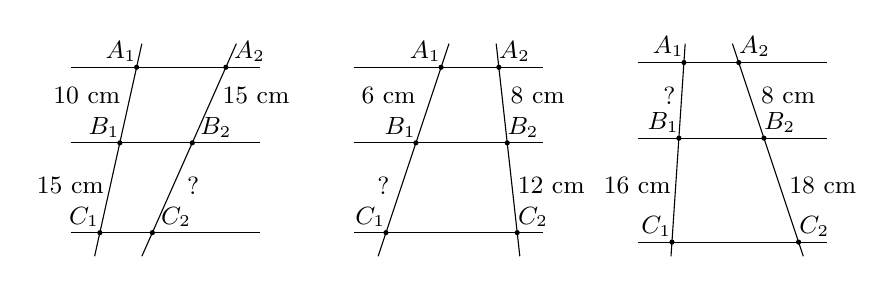
\begin{tikzpicture}[scale=0.6,font=\small]
\usetikzlibrary{calc}

\begin{scope}
\coordinate (a1) at (0,0);
\coordinate (a2) at (4,0);
\coordinate (b1) at (0,-1.6);
\coordinate (b2) at (4,-1.6);
\coordinate (c1) at (0,-3.5);
\coordinate (c2) at (4,-3.5);
\coordinate (t11) at (1.5,0.5);
\coordinate (t12) at (0.5,-4);
\coordinate (t21) at (3.5,0.5);
\coordinate (t22) at (1.5,-4);
\coordinate (A1) at (intersection of a1--a2 and t11--t12);
\coordinate (A2) at (intersection of a1--a2 and t21--t22);
\coordinate (B1) at (intersection of b1--b2 and t11--t12);
\coordinate (B2) at (intersection of b1--b2 and t21--t22);
\coordinate (C1) at (intersection of c1--c2 and t11--t12);
\coordinate (C2) at (intersection of c1--c2 and t21--t22);

\draw (a1) -- (a2);
\draw (b1) -- (b2);
\draw (c1) -- (c2);
\draw (t11) -- (t12);
\draw (t21) -- (t22);
\draw[fill] (A1) circle (1.2pt) node[shift={(-0.2,0.2)}] {$A_1$};
\draw[fill] (A2) circle (1.2pt) node[shift={(0.3,0.2)}] {$A_2$};
\draw[fill] (B1) circle (1.2pt) node[shift={(-0.2,0.2)}] {$B_1$};
\draw[fill] (B2) circle (1.2pt) node[shift={(0.3,0.2)}] {$B_2$};
\draw[fill] (C1) circle (1.2pt) node[shift={(-0.2,0.2)}] {$C_1$};
\draw[fill] (C2) circle (1.2pt) node[shift={(0.3,0.2)}] {$C_2$};

\node[left] at (1.25, -0.6) {10 cm};
\node[left] at (0.9, -2.5) {15 cm};
\node[right] at (3, -0.6) {15 cm};
\node[right] at (2.25, -2.5) {?};

\end{scope}



\begin{scope}[xshift=6cm]
\coordinate (a1) at (0,0);
\coordinate (a2) at (4,0);
\coordinate (b1) at (0,-1.6);
\coordinate (b2) at (4,-1.6);
\coordinate (c1) at (0,-3.5);
\coordinate (c2) at (4,-3.5);
\coordinate (t11) at (2,0.5);
\coordinate (t12) at (0.5,-4);
\coordinate (t21) at (3,0.5);
\coordinate (t22) at (3.5,-4);
\coordinate (A1) at (intersection of a1--a2 and t11--t12);
\coordinate (A2) at (intersection of a1--a2 and t21--t22);
\coordinate (B1) at (intersection of b1--b2 and t11--t12);
\coordinate (B2) at (intersection of b1--b2 and t21--t22);
\coordinate (C1) at (intersection of c1--c2 and t11--t12);
\coordinate (C2) at (intersection of c1--c2 and t21--t22);

\draw (a1) -- (a2);
\draw (b1) -- (b2);
\draw (c1) -- (c2);
\draw (t11) -- (t12);
\draw (t21) -- (t22);
\draw[fill] (A1) circle (1.2pt) node[shift={(-0.2,0.2)}] {$A_1$};
\draw[fill] (A2) circle (1.2pt) node[shift={(0.2,0.2)}] {$A_2$};
\draw[fill] (B1) circle (1.2pt) node[shift={(-0.2,0.2)}] {$B_1$};
\draw[fill] (B2) circle (1.2pt) node[shift={(0.2,0.2)}] {$B_2$};
\draw[fill] (C1) circle (1.2pt) node[shift={(-0.2,0.2)}] {$C_1$};
\draw[fill] (C2) circle (1.2pt) node[shift={(0.2,0.2)}] {$C_2$};

\node[left] at (1.5, -0.6) {6 cm};
\node[left] at (0.95, -2.5) {?};
\node[right] at (3.1, -0.6) {8 cm};
\node[right] at (3.25, -2.5) {12 cm};

\end{scope}



\begin{scope}[xshift=12cm]
\coordinate (a1) at (0,0.1);
\coordinate (a2) at (4,0.1);
\coordinate (b1) at (0,-1.5);
\coordinate (b2) at (4,-1.5);
\coordinate (c1) at (0,-3.7);
\coordinate (c2) at (4,-3.7);
\coordinate (t11) at (1,0.5);
\coordinate (t12) at (0.7,-4);
\coordinate (t21) at (2,0.5);
\coordinate (t22) at (3.5,-4);
\coordinate (A1) at (intersection of a1--a2 and t11--t12);
\coordinate (A2) at (intersection of a1--a2 and t21--t22);
\coordinate (B1) at (intersection of b1--b2 and t11--t12);
\coordinate (B2) at (intersection of b1--b2 and t21--t22);
\coordinate (C1) at (intersection of c1--c2 and t11--t12);
\coordinate (C2) at (intersection of c1--c2 and t21--t22);

\draw (a1) -- (a2);
\draw (b1) -- (b2);
\draw (c1) -- (c2);
\draw (t11) -- (t12);
\draw (t21) -- (t22);
\draw[fill] (A1) circle (1.2pt) node[shift={(-0.2,0.2)}] {$A_1$};
\draw[fill] (A2) circle (1.2pt) node[shift={(0.2,0.2)}] {$A_2$};
\draw[fill] (B1) circle (1.2pt) node[shift={(-0.2,0.2)}] {$B_1$};
\draw[fill] (B2) circle (1.2pt) node[shift={(0.2,0.2)}] {$B_2$};
\draw[fill] (C1) circle (1.2pt) node[shift={(-0.2,0.2)}] {$C_1$};
\draw[fill] (C2) circle (1.2pt) node[shift={(0.2,0.2)}] {$C_2$};

\node[left] at (1, -0.6) {?};
\node[left] at (0.9, -2.5) {16 cm};
\node[right] at (2.4, -0.6) {8 cm};
\node[right] at (3, -2.5) {18 cm};

\end{scope}

\end{tikzpicture}

	\caption{Esercizio~\ref{ese:6.31}}\label{fig:ese6.31}
\end{figure}

\noindent\begin{minipage}{0.6\textwidth}\parindent15pt
\begin{esercizio}
\label{ese:6.32}
Con riferimento alla figura a fianco, quali proporzioni sono conseguenza del teorema di Talete?
\begin{enumeratea}
\item $u : v = m : n$
\item $u : m = v : n$
\item $(u+m) : m = (v+n) : n$
\item $v : m = u : n$
\item $(u + v) : (m + n) = m : n$
\item $(m-u) : u = (n-v) : v$
\end{enumeratea}
\end{esercizio}
\end{minipage}\hfil
\begin{minipage}{0.4\textwidth}
	\centering% Copyright (c) 2015 Daniele Masini - d.masini.it@gmail.com

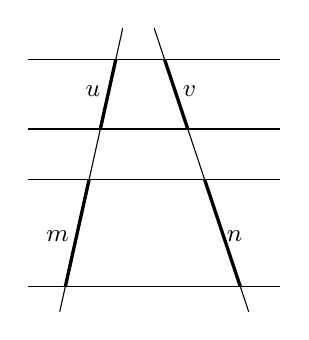
\begin{tikzpicture}[scale=0.8,font=\small]
\usetikzlibrary{calc}

\begin{scope}
\coordinate (a1) at (0,0);
\coordinate (a2) at (4,0);
\coordinate (b1) at (0,-1.1);
\coordinate (b2) at (4,-1.1);
\coordinate (c1) at (0,-1.9);
\coordinate (c2) at (4,-1.9);
\coordinate (d1) at (0,-3.6);
\coordinate (d2) at (4,-3.6);
\coordinate (t11) at (1.5,0.5);
\coordinate (t12) at (0.5,-4);
\coordinate (t21) at (2,0.5);
\coordinate (t22) at (3.5,-4);
\coordinate (A1) at (intersection of a1--a2 and t11--t12);
\coordinate (A2) at (intersection of a1--a2 and t21--t22);
\coordinate (B1) at (intersection of b1--b2 and t11--t12);
\coordinate (B2) at (intersection of b1--b2 and t21--t22);
\coordinate (C1) at (intersection of c1--c2 and t11--t12);
\coordinate (C2) at (intersection of c1--c2 and t21--t22);
\coordinate (D1) at (intersection of d1--d2 and t11--t12);
\coordinate (D2) at (intersection of d1--d2 and t21--t22);

\draw (a1) -- (a2);
\draw (b1) -- (b2);
\draw (c1) -- (c2);
\draw (d1) -- (d2);
\draw (t11) -- (t12);
\draw (t21) -- (t22);

\draw[very thick] (A1) -- (B1);
\draw[very thick] (C1) -- (D1);
\draw[very thick] (A2) -- (B2);
\draw[very thick] (C2) -- (D2);

\node[left] at (1.3, -0.5) {$u$};
\node[left] at (0.8, -2.8) {$m$};
\node[right] at (2.3, -0.5) {$v$};
\node[right] at (3, -2.8) {$n$};

\end{scope}

\end{tikzpicture}

\end{minipage}\vspace{4pt}

\noindent\begin{minipage}{0.6\textwidth}\parindent15pt
\begin{esercizio}
\label{ese:6.33}
Nella figura a fianco c'è un triangolo e una delle sue bisettrici. Quali proporzioni sono conseguenza del teorema della bisettrice?
\begin{enumeratea}
\item $a : b = x : y$
\item \ldots{}
\item \ldots{}
\item \ldots{}
\end{enumeratea}
\end{esercizio}
\end{minipage}\hfil
\begin{minipage}{0.4\textwidth}
	\centering% (c) 2014 Daniele Masini - d.masini.it@gmail.com
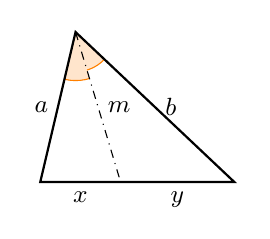
\begin{tikzpicture}[scale=0.8,font=\small]
\usetikzlibrary{calc}

\clip (-0.2,-0.45) rectangle (3.2,2.45);

\begin{scope}[scale=1.4]
\coordinate (a) at (0,0);
\coordinate (c) at (0.4,1.7);
\coordinate (b) at (2.2,0);

\path (c) let \p1 = ($(b)-(c)$) in -- ($(c)!{veclen(\x1,\y1)}!(a)$) -- +($(b)-(c)$) coordinate (c1);
\coordinate (d) at (intersection of c--c1 and a--b);

\begin{scope}
\clip (c) -- (a) -- (d) -- cycle;
\draw[orange, fill=orange!20] (c) circle (0.55);
\end{scope}

\begin{scope}
\clip (c) -- (d) -- (b) -- cycle;
\draw[orange, fill=orange!20] (c) circle (0.45);
\end{scope}


\draw[dashdotted] (c) -- node[right] {$m$} (d);
\draw[thick] (a) -- (b) -- node[right] {$b$} (c) -- cycle;
\path (a) -- node[left] {$a$} (c);
\path (a) -- node[below] {$x$} (d);
\path (d) -- node[below] {$y$} (b);

\end{scope}


\end{tikzpicture}

\end{minipage}

\noindent\begin{minipage}{0.6\textwidth}\parindent15pt
\begin{esercizio}
\label{ese:6.34}
Sapendo che le rette $r$, $s$, $t$ e $u$ della figura a fianco sono parallele, completa le proporzioni
\begin{enumeratea}
\item $AB : CD = \ldots{} : \ldots{}$
\item $AC : BD = \ldots{} : \ldots{}$
\item $AB : \ldots{} = \ldots{} : B'C'$
\item $AC : A'C' = \ldots{} : \ldots{}$
\end{enumeratea}
\end{esercizio}
\end{minipage}\hfil
\begin{minipage}{0.4\textwidth}
	\centering% Copyright (c) 2015 Daniele Masini - d.masini.it@gmail.com

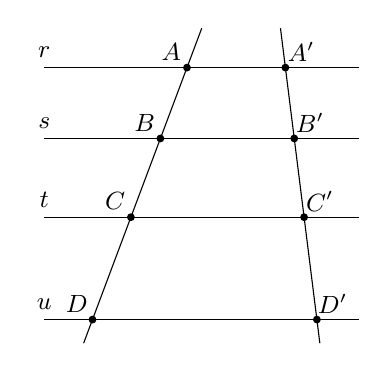
\begin{tikzpicture}[scale=1,font=\small]
\usetikzlibrary{calc}

\begin{scope}
\coordinate (a1) at (0,0);
\coordinate (a2) at (4,0);
\coordinate (b1) at (0,-.9);
\coordinate (b2) at (4,-.9);
\coordinate (c1) at (0,-1.9);
\coordinate (c2) at (4,-1.9);
\coordinate (d1) at (0,-3.2);
\coordinate (d2) at (4,-3.2);
\coordinate (t11) at (2,0.5);
\coordinate (t12) at (0.5,-3.5);
\coordinate (t21) at (3,0.5);
\coordinate (t22) at (3.5,-3.5);
\coordinate (A1) at (intersection of a1--a2 and t11--t12);
\coordinate (A2) at (intersection of a1--a2 and t21--t22);
\coordinate (B1) at (intersection of b1--b2 and t11--t12);
\coordinate (B2) at (intersection of b1--b2 and t21--t22);
\coordinate (C1) at (intersection of c1--c2 and t11--t12);
\coordinate (C2) at (intersection of c1--c2 and t21--t22);
\coordinate (D1) at (intersection of d1--d2 and t11--t12);
\coordinate (D2) at (intersection of d1--d2 and t21--t22);

\draw (a1) node[above] {$r$} -- (a2);
\draw (b1) node[above] {$s$} -- (b2);
\draw (c1) node[above] {$t$} -- (c2);
\draw (d1) node[above] {$u$} -- (d2);
\draw (t11) -- (t12);
\draw (t21) -- (t22);
\draw[fill] (A1) circle (1.2pt) node[shift={(-0.2,0.2)}] {$A$};
\draw[fill] (A2) circle (1.2pt) node[shift={(0.2,0.2)}] {$A'$};
\draw[fill] (B1) circle (1.2pt) node[shift={(-0.2,0.2)}] {$B$};
\draw[fill] (B2) circle (1.2pt) node[shift={(0.2,0.2)}] {$B'$};
\draw[fill] (C1) circle (1.2pt) node[shift={(-0.2,0.2)}] {$C$};
\draw[fill] (C2) circle (1.2pt) node[shift={(0.2,0.2)}] {$C'$};
\draw[fill] (D1) circle (1.2pt) node[shift={(-0.2,0.2)}] {$D$};
\draw[fill] (D2) circle (1.2pt) node[shift={(0.2,0.2)}] {$D'$};

\end{scope}

\end{tikzpicture}

\end{minipage}

\begin{multicols}{2}

\begin{esercizio}
\label{ese:6.35}
Nel triangolo $ABC$, individua sul lato $AB$ i punti $D$ ed $E$, con $D$ più vicino ad $A$. Da $D$ ed $E$ traccia le parallele sia al lato $AC$ che al lato $BC$, come in figura~\ref{fig:ese6.35}. Dimostra che sussiste la seguente proporzione $AC:BC=FG:HI$.
\end{esercizio}

\begin{figure}[!htb]
	\centering% Copyright (c) 2015 Daniele Masini - d.masini.it@gmail.com

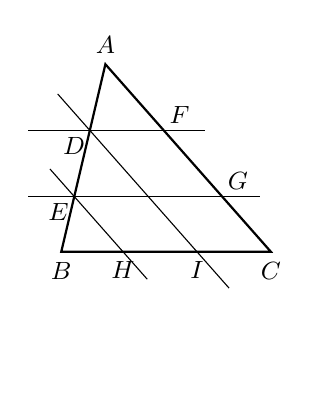
\begin{tikzpicture}[scale=1.4,font=\small]
\usetikzlibrary{calc}

%\clip (-0.2,-0.45) rectangle (3.2,2.45);

\begin{scope}
\coordinate (b) at (0,0);
\coordinate (a) at (0.4,1.7);
\coordinate (c) at (1.9,0);
\coordinate (r1) at (-0.3,1.1);
\coordinate (r2) at (1.3,1.1);
\coordinate (s1) at (-0.3,0.5);
\coordinate (s2) at (1.8,0.5);

\coordinate (d) at (intersection of r1--r2 and a--b);
\coordinate (f) at (intersection of r1--r2 and a--c);
\coordinate (e) at (intersection of s1--s2 and a--b);
\coordinate (g) at (intersection of s1--s2 and a--c);

\node[shift={(-.2,-.2)}] at (d) {$D$};
\node[shift={(-.2,-.2)}] at (e) {$E$};
\node[shift={(.2,.2)}] at (f) {$F$};
\node[shift={(.2,.2)}] at (g) {$G$};
\path (d) -- +($(c)-(a)$) coordinate (t2);
\path (e) -- +($(c)-(a)$) coordinate (u2);


\coordinate (i) at (intersection of d--t2 and b--c);
\coordinate (h) at (intersection of e--u2 and b--c);

\node[below] at (h) {$H$};
\node[below] at (i) {$I$};

\draw (r1) -- (r2);
\draw (s1) -- (s2);
\draw ($(d)!-0.3!(i)$) -- ($(d)!1.3!(i)$);
\draw ($(e)!-0.5!(h)$) -- ($(e)!1.5!(h)$);
\draw[thick] (a) node[above] {$A$} -- (b) node[below] {$B$} --(c) node[below] {$C$} -- cycle;
%\path (a) -- node[left] {$a$} (c);
%\path (a) -- node[below] {$x$} (d);
%\path (d) -- node[below] {$y$} (b);

\end{scope}


\end{tikzpicture}

	\caption{Esercizio~\ref{ese:6.35}}\label{fig:ese6.35}
\end{figure}

\begin{esercizio}
\label{ese:6.36}
Dato un triangolo qualunque $ABC$, si consideri il punto medio $M$ del lato $AB$. Si consideri il segmento parallelo al lato $BC$ che parte da $M$ ed incontra il lato $AC$ nel punto $N$. Si prolunghi questo segmento di un segmento $ND$ uguale ad $MN$. Dimostra che il quadrilatero $MDCB$ è un parallelogramma. Esplicita ipotesi, tesi, fai il disegno e dimostra la tesi.
\end{esercizio}

\begin{esercizio}
\label{ese:6.37}
Dato un parallelogramma $ABCD$, si consideri $M$ il punto medio del lato $AB$. Si congiunga il vertice $D$ con il punto $M$; si congiunga il vertice $A$ con il punto medio $N$ del segmento $DM$. Dimostra che la retta $AN$ divide la diagonale $DB$ del parallelogramma in due parti di cui una è il doppio dell'altra.
\end{esercizio}

\begin{esercizio}
\label{ese:6.38}
Due rette incidenti $r$ ed $s$ si incontrano in un punto $A$; sulla retta $r$ considera i punti $A'$ e $A''$, individua su $s$ le proiezioni ortogonali di $A'$ e $A''$ e chiama questi punti rispettivamente $B'$ e $B''$. Dimostra che sussiste la seguente proporzione $AA' : AA'' = BB' : BB''$.
\end{esercizio}

\begin{esercizio}
\label{ese:6.39}
Dal baricentro $G$ di un triangolo $ABC$ manda la parallela al lato $AB$, sia $A'$ il punto in cui questa parallela incontra il lato $AC$. Dimostra che $CA'$ è il doppio di $A'A$. Ricorda le proprietà del baricentro.
\end{esercizio}

\begin{esercizio}
\label{ese:6.40}
Dato il trapezio $ABCD$, sia $E$ il punto di intersezione dei due lati non paralleli $AD$ e $BC$. Dimostra che una qualsiasi retta per $E$ che incontri i lati paralleli del trapezio nei punti $K$ ed $L$, determina due segmenti $EK$ e $KL$ il cui rapporto è costante.
\end{esercizio}

\begin{esercizio}
\label{ese:6.41}
Dimostrare che, in un trapezio, il segmento che congiunge i punti medi dei lati non paralleli è uguale alla semisomma delle basi.
\end{esercizio}

\begin{esercizio}
\label{ese:6.42}
Nel parallelogramma $ABCD$ si individuino il punto $E$ su $AB$ tale che $AB : AE = 3 : 2$ e il punto $F$ su $DC$ tale che $DC : FC = 3 : 2$. Traccia la diagonale $DB$ e le rette $AF$ ed $EC$, le quali intersecano $DB$ rispettivamente in $L$ e in $M$. A quali numeri sono proporzionali i segmenti $DL$, $LM$ e $MB$?
\end{esercizio}

\begin{esercizio}
\label{ese:6.43}
Dimostra che nel triangolo $ABC$ la mediana $AM$ è il luogo dei punti medi delle parallele al lato $BC$.
\end{esercizio}

\begin{esercizio}
\label{ese:6.44}
Nel triangolo $ABC$ prendi un punto qualsiasi $D$ su $AB$, da $D$ traccia la parallela ad $AC$ che incontra $BC$ in $E$, da $E$ traccia la parallela ad $AB$ che incontra $AC$ in $F$, da $F$ traccia la parallela a $BC$ che incontra $AB$ in $G$, da $G$ la parallela ad $AC$ che incontra $BC$ in $H$, da $H$ la parallela ad $AB$ che incontra $AC$ in $I$ e così via. Ripeti questa costruzione fino a che non trovi il primo punto che va a sovrapporsi a uno dei punti trovati in precedenza. Esiste questo punto? Qual è? Dimostra perché.
\end{esercizio}

\begin{esercizio}
\label{ese:6.45}
Nel triangolo $ABC$ traccia la bisettrice $AK$ dell'angolo in $A$. Sapendo che la somma dei lati adiacenti all'angolo misura 47~cm, che $BK : CK = 3 : 4$ e che $BK$ misura 7~cm, determinare le misure dei lati del triangolo.
\end{esercizio}

\begin{esercizio}
\label{ese:6.46}
Dal punto $K$ della mediana $AM$ del triangolo $ABC$ traccia le parallele ai tre lati del triangolo, siano $D$ ed $E$ i punti di intersezione di $AB$ e $AC$ con la parallela a $BC$, siano $F$ e $G$ i punti di intersezione delle altre due parallele con il lato $BC$. Dimostra che $AK$ è mediana del triangolo $ADE$ e che $KM$ è la mediana del triangolo $KFG$.
\end{esercizio}

\begin{esercizio}
\label{ese:6.47}
Sia $E$ il punto di intersezione delle diagonali del trapezio $ABCD$. Dimostra che $AE : EC = BE : ED$.
\end{esercizio}

\begin{esercizio}
\label{ese:6.48}
Dimostra che in qualsiasi triangolo $ABC$ la retta che passa per i punti medi dei lati $AB$ e $AC$ divide in due parti uguali l'altezza relativa a $BC$.
\end{esercizio}

\begin{esercizio}
\label{ese:6.49}
In un triangolo $ABC$ sia $AB<AC$ e $AM$ la mediana relativa al lato $BC$. Sia $N$ punto medio di $BM$. Conduci da $N$ la parallela alla mediana $AM$ che incontra la retta $AB$ in $P$ e la retta $AC$ in $Q$. Dimostra che $AQ : AC = AP : AB$.
\end{esercizio}

\begin{esercizio}
\label{ese:6.50}
Dimostra che in un qualsiasi trapezio le diagonali si dividono scambievolmente in parti tra loro direttamente proporzionali.
\end{esercizio}

\subsubsection*{\thechapter.4 - Avere la stessa forma}

\begin{esercizio}
\label{ese:6.51}
In un trapezio congiungi i punti medi dei lati obliqui, sono simili i due trapezi in cui quello dato risulta spezzato dalla congiungente tracciata? 
\end{esercizio}

\begin{esercizio}
\label{ese:6.52}
Congiungi i punti medi $M$, $N$, $P$ rispettivamente dei lati $AB$, $AC$ e $BC$ di un triangolo $ABC$ e determina il valore di verità della proposizione: $MNP\sim ABC$ con rapporto di similitudine $\np{0,5}$.
\end{esercizio}

\begin{esercizio}
\label{ese:6.53}
\`E vero che due poligoni regolari aventi lo stesso numero di lati sono simili? Giustifica la risposta.
\end{esercizio}

\begin{esercizio}
\label{ese:6.54}
Assegnato il quadrato $MNPQ$, costruisci il quadrato $M’N’P’Q’$ la cui diagonale sia doppia della diagonale $MP$. \`E vero che $M’N’P’Q’\sim MNPQ$? Qual è il rapporto di similitudine? Costruisci il quadrato $M''N''P''Q''$ avente diagonale metà di $MP$. \`E vero che $M''N''P''Q''\sim MNPQ$? Qual è il rapporto di similitudine? \`E vero che tra le aree dei tre quadrati valgono le seguenti relazioni?
\[A_{MNPQ}=\frac{1}{2}A_{M'N'P'Q'}=2A_{M''N''P''Q''} \]
\end{esercizio}

\begin{esercizio}
\label{ese:6.55}
Verifica che la relazione ``essere simili'' nell'insieme dei poligoni è una relazione di equivalenza (gode cioè della proprietà riflessiva, simmetrica e transitiva).
\end{esercizio}

\subsubsection*{\thechapter.5 - La similitudine nei triangoli}

\begin{esercizio}
\label{ese:6.56}
Dimostra che la parallela ad un lato di un triangolo che interseca gli altri due determina un triangolo simile a quello dato. Scrivi la proporzione che sussiste tra i lati.
\end{esercizio}

\begin{esercizio}
\label{ese:6.57}
Nel triangolo isoscele $ABC$ di vertice $A$, traccia la mediana $AM$ e dal punto $M$ traccia la perpendicolare al lato obliquo $AB$. Individua tutti i triangoli simili che si vengono a formare nella figura.
\end{esercizio}

\begin{esercizio}
\label{ese:6.58}
Nel triangolo $ABC$ traccia l'altezza $AH$ relativa al lato $BC$ e l'altezza $CK$ relativa al lato $AB$. Individua tutti i triangoli simili che si vengono a formare nella figura.
\end{esercizio}

\begin{esercizio}
\label{ese:6.59}
Nel triangolo rettangolo $ABC$, rettangolo in $B$, traccia la bisettrice $AL$ e da $L$ la perpendicolare all'ipotenusa $AC$. Individua tutti i triangoli simili che si vengono a formare nella figura.
\end{esercizio}

\begin{esercizio}
\label{ese:6.60}
Nel trapezio $ABCD$ di basi $AB$ e $CD$, detto $P$ il punto d'incontro delle diagonali, risultano simili i triangoli $ABP$ e $CDP$. Se le basi sono una doppia dell'altra, concludete la proposizione: <<il punto $P$ divide ciascuna diagonale in \ldots\ldots\ldots{}>>
\end{esercizio}

\begin{esercizio}
\label{ese:6.61}
Dal punto $K$ dell'ipotenusa $BC$ del triangolo rettangolo $ABC$ tracciate la perpendicolare all'ipotenusa stessa che incontra le rette dei cateti $AC$ e $AB$ rispettivamente nei punti $F$ e $G$. Dimostrate che: $FKC\sim FAG$ e $GKB\sim GAF$. Se $AC:AB=7:5$ è vero che lo stesso rapporto sussiste tra i cateti dei triangoli nominati?
\end{esercizio}

\begin{esercizio}
\label{ese:6.62}
Nel trapezio rettangolo $ABCD$ con $AD$ perpendicolare alle basi, la diagonale minore $AC$ è perpendicolare al lato obliquo $BC$. Dimostrate che i due triangoli in cui la diagonale divide il trapezio sono simili. Nella prima riga della seguente tabella abbiamo posto i lati di un triangolo; Completate la seconda riga con i lati omologhi dell'altro triangolo e quindi la proporzione $CB:\ldots{}=AC:\ldots{}=AB:\ldots{}$.

\begin{center}
\begin{tabular}{cccc}
\toprule
$ABC$ & $CB$ & $AC$ & $AB$\\
$ADC$ & \ldots{} & \ldots{} & \ldots{}\\
\bottomrule
\end{tabular}
\end{center}
\end{esercizio}

\begin{esercizio}
\label{ese:6.63}
$ABC$ e $A'B'C'$ sono due triangoli simili, $CR$ e $C'R'$ sono le bisettrici rispettivamente degli angoli $\widehat{C}$ e $\widehat{C'}$ ($R\in AB$ e $R\in A'B'$). Dimostrate che $CR : C'R' = AB : A'B'$. Se $CR$ e $C'R'$ sono rispettivamente le altezze relative ad $AB$ e $A'B'$, vale la stessa proporzione? \`E possibile dimostrare, utilizzando il primo criterio di similitudine, che tale proporzione sussiste anche se $CR$ e $C'R'$ fossero le mediane relative ad $AB$ e $A'B'$?
\end{esercizio}

\begin{esercizio}
\label{ese:6.64}
In un trapezio $ABCD$ di basi $AB=4$~cm, $DC=8$~cm, traccia le diagonali $AC$ e $BD$ sapendo che esse misurano rispettivamente \np{7,62}~cm e \np{5,83}~cm. Indicato con $K$ il punto di intersezione delle diagonali, determina le misure in cui ciascuna diagonale resta divisa dall'altra. [\np{2,54}; \np{5,08}; \np{3,89}; \np{1,94}]
\end{esercizio}

\begin{esercizio}
\label{ese:6.65}
Nel triangolo $ABC$ traccia le altezze $AH$ e $BK$. Dimostra che il triangolo $4CHK$ è simile al triangolo $ABC$. Osserva che $BKA$ e $AHB$ sono inscrivibili in una semicirconferenza.
\end{esercizio}

\begin{esercizio}
\label{ese:6.66}
Siano $BH$ e $CK$ due altezze del triangolo $ABC$. Dimostra che $AKH$ è simile ad $ABC$. Osserva che $BCK$ e $BCH$ sono inscrivibili in una semicirconferenza.
\end{esercizio}

\begin{esercizio}
\label{ese:6.67}
Un trapezio ha le basi di 4~cm e 10~cm, i lati obliqui di \np{4,57}~cm e \np{5,94}~cm. Prolungandoli si ottiene un triangolo che ha in comune con il trapezio la base minore. Determina il perimetro del triangolo. [R.~\np{21,52}~cm].
\end{esercizio}

\begin{esercizio}
\label{ese:6.68}
Dimostra che due triangoli sono simili se hanno i lati del primo triangolo rispettivamente perpendicolari ai lati del secondo triangolo. 
\end{esercizio}

\begin{esercizio}
\label{ese:6.69}
In un trapezio rettangolo la base minore $CD$ è doppia del lato obliquo $BC$ e questo è i $5/4$ del lato $AD$ perpendicolare alle due basi. Sapendo che l'area del trapezio è 184~cm\textsuperscript{2}, calcolare la misura della distanza di $D$ dalla retta $BC$. [16~cm] 
\end{esercizio}

\begin{esercizio}
\label{ese:6.70}
Nel triangolo $ABC$, traccia da un punto $M$ del lato $AB$ la parallela a $BC$; essa incontra $AC$ in $N$. Traccia poi la bisettrice $AL$ del triangolo; essa incontra $MN$ in $K$. Dimostra che $AMK$ è simile ad $ABL$.
\end{esercizio}

\begin{esercizio}
\label{ese:6.71}
Da un punto $P$ dell'ipotenusa $BC$ del triangolo rettangolo $ABC$ invia le parallele ai cateti del triangolo. Esse individuano $Q$ au $AB$ e $R$ su $AC$. Dimostra che sono simili i triangoli $ABC$, $QBP$ e $RPC$.
\end{esercizio}

\begin{esercizio}
\label{ese:6.72}
Due circonferenze, di centri $O$ ed $O'$ e raggi di misura rispettivamente 6~cm e 12~cm, sono tra loro tangenti esternamente in $A$; da $O$ si tracci una tangente alla circonferenza di centro $O'$ e sia $B$ il punto di tangenza. Indicato con $M$ il punto in cui il segmento $BO$ incontra la circonferenza di centro $O$, calcolare le misure dei lati del triangolo $AOM$. [6~cm, 4~cm, \ldots{}]
\end{esercizio}

\begin{esercizio}
\label{ese:6.73}
Il rapporto tra l'altezza $AH$ e la base $BC$ del triangolo isoscele $ABC$ è $2:3$. Indicata con $D$ la proiezione ortogonale di $C$ sulla retta $AB$, dimostrare che $D$ è un punto interno al segmento $AB$. Si costruisca poi il triangolo $ECD$, isoscele su base $CD$ e simile ad $ABC$, in modo che il punto $E$ si trovi dalla stessa parte di $A$ rispetto a $BC$. Si dimostri che $CE$ è parallelo ad $AH$, che i triangoli $CDB$ e $CEA$ sono simili e che il quadrilatero $ECDA$ è inscrivibile in una circonferenza.
\end{esercizio}

\begin{esercizio}
\label{ese:6.74}
Dimostrate che in due triangoli simili le mediane relative a due lati omologhi rispettano il rapporto di similitudine.
\end{esercizio}

\begin{esercizio}
\label{ese:6.75}
Due segmenti $AB$ e $CD$ si tagliano in un punto $P$ in modo che $AP:PD=CP:PB$. Dimostra che $\widehat{A}\cong \widehat{D}$ e $\widehat{B}\cong \widehat{C}$.
\end{esercizio}

\begin{esercizio}
\label{ese:6.76}
Sui segmenti consecutivi $AB$ e $AC$ si prendano rispettivamente i punti $H$ e $K$ in modo che $AH\cong \frac{3}{4}AB$ e $AK\cong \frac{3}{4}AC$. Dimostrate che $HK$ è parallelo a $BC$.
\end{esercizio}

\begin{esercizio}
\label{ese:6.77}
Prolungate, dalla parte di $A$, i lati congruenti $AB$ e $AC$ del triangolo isoscele $ABC$, di due segmenti congruenti $AE$ e $AF$. Dimostrate che $FE$ è parallelo a $BC$.
\end{esercizio}

\begin{esercizio}
\label{ese:6.78}
Da un punto $A$ su una circonferenza traccia le corde $AB$ e $AC$. Prolunga quindi $AB$ di un segmento $BD$ pari alla metà di $AB$ e prolunga $AC$ di un segmento $CE$ pari alla metà di $AC$. Dimostra che il triangolo $ABC$ è simile al triangolo $ADE$.
\end{esercizio}

\begin{esercizio}
\label{ese:6.79}
In quali dei seguenti casi due triangoli sono simili?
\begin{enumeratea}
\item se hanno due coppie di lati in proporzione\tab\hfill\boxV\quad\boxF
\item se hanno due coppie di angoli in proporzione\tab\hfill\boxV\quad\boxF
\item se hanno due coppie di angoli congruenti\tab\hfill\boxV\quad\boxF
\item se hanno una coppia di lati in proporzione e una coppia di angoli congruenti\tab\hfill\boxV\quad\boxF
\item se sono rettangoli e hanno un angolo acuto congruente\hfill\boxV\quad\boxF
\end{enumeratea}
\end{esercizio}

\begin{esercizio}
\label{ese:6.80}
I lati del triangolo $ABC$ misurano $AB=8$~cm, $AC=\np{7,5}$~cm e $BC=5$~cm. A che distanza da $B$ bisogna prendere sul lato $BC$ un punto $D$ in modo che la somma di $DF$ parallelo a $BA$ e $DE$ parallelo a $CA$ sia \np{7,8}~cm? Individua i triangoli simili.	[R.~$DB=2$~cm]
\end{esercizio}

\begin{esercizio}
\label{ese:6.81}
In un trapezio $ABCD$ di basi $AB=3$~cm e $DC=7$~cm, traccia le diagonali $AC$ e $BD$ e indica con $E$ il punto di intersezione delle diagonali. Da $E$ traccia la parallela alle basi del trapezio e indica con $F$ e $G$ i punti di intersezione di questa parallela con i lati obliqui $AD$ e $BC$. Determina la lunghezza di $FG$. ($ABE\sim DEC$, $AFE\sim ADC$, \ldots). [R.~\np{4,2}~cm]
\end{esercizio}

\begin{esercizio}
\label{ese:6.82}
Dimostra che due triangoli sono simili se hanno le mediane che sono proporzionali.
\end{esercizio}

\begin{esercizio}
\label{ese:6.83}
Dimostra che congiungendo i punti medi di un triangolo equilatero si ottiene un triangolo equilatero simile.
\end{esercizio}

\begin{esercizio}
\label{ese:6.84}
Nel trapezio $ABCD$ rettangolo in $A$ e in $D$, le diagonali $BD$ e $AC$ sono perpendicolari. Sapendo che $AB=3$~cm, $AD=4$~cm e $BD=5$~cm, calcola la lunghezza della base maggiore $DC$. (Utilizza la similitudine dei triangoli $ABD$ e \ldots{})	[R.~\np{5,33}~cm]
\end{esercizio}

\begin{esercizio}
\label{ese:6.85}
Il rapporto fra le basi di due triangoli isosceli è $2/5$ e la somma delle loro aree è 435~cm\textsuperscript{2}; sapendo che l'altezza relativa alla base del primo triangolo misura 10~cm, calcolare i perimetri dei due triangoli. 
\end{esercizio}

\begin{esercizio}
\label{ese:6.86}
Due triangoli $ABC$ e $DEF$ (figura~\ref{fig:ese6.86}) hanno le basi $AB$ e $DF$ e i vertici $C$ ed $E$ su rette parallele. Dimostrate che $IJ:KL=AB:DF$, dove $IJ$ e $KL$ sono le corde intercettate dai lati dei due triangoli su una retta parallela alle basi (tracciate le altezze $CP$ e $EQ$).
\end{esercizio}

\begin{figure}[!htb]
	\centering% Copyright (c) 2015 Daniele Masini - d.masini.it@gmail.com

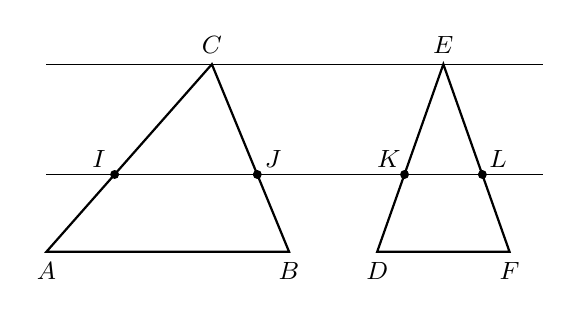
\begin{tikzpicture}[scale=1.4,font=\small]
\usetikzlibrary{calc}


\begin{scope}
\coordinate (c) at (1.5,1.7);
\coordinate (a) at (0,0);
\coordinate (b) at (2.2,0);


\draw[thick] (a) node[below] {$A$} -- (b) node[below] {$B$} -- (c) node[above] {$C$} -- cycle;

\end{scope}


\begin{scope}[xshift=3cm]
\coordinate (e) at (0.6,1.7);
\coordinate (d) at (0,0);
\coordinate (f) at (1.2,0);
\draw[thick] (d) node[below] {$D$} -- (f) node[below] {$F$} -- (e) node[above] {$E$} -- cycle;

\end{scope}

\coordinate (r1) at (0,0.7);
\coordinate (r2) at (4.5,0.7);
\coordinate (s1) at (0,1.7);
\coordinate (s2) at (4.5,1.7);
\coordinate (i) at (intersection of r1--r2 and a--c);
\coordinate (j) at (intersection of r1--r2 and b--c);
\coordinate (k) at (intersection of r1--r2 and d--e);
\coordinate (l) at (intersection of r1--r2 and e--f);

\draw (r1) -- (r2);
\draw (s1) -- (s2);

\draw[fill] (i) circle (1pt) node[shift={(-.2,.2)}] {$I$};
\draw[fill] (j) circle (1pt) node[shift={(.2,.2)}] {$J$};
\draw[fill] (k) circle (1pt) node[shift={(-.2,.2)}] {$K$};
\draw[fill] (l) circle (1pt) node[shift={(.2,.2)}] {$L$};

\end{tikzpicture}

	\caption{Esercizio~\ref{ese:6.86}}\label{fig:ese6.86}
\end{figure}

\begin{esercizio}
\label{ese:6.87}
Se in un trapezio il rapporto tra le basi è $\frac{2}{7}$ e l'altezza è di 18~m, determinate la misura delle due parti nelle quali l'altezza risulta divisa dal punto di intersezione delle diagonali. Quanto dista dalla base minore il punto d'incontro dei lati obliqui del trapezio?  [R.~$h_1=4$~m; $h_2=14$~m; $d=\np{7,2}$~m]
\end{esercizio}

\begin{esercizio}
\label{ese:6.88}
Il rapporto tra le aree dei due triangoli simili $ABC$ e $A'B'C'$ è $\frac{25}{9}$ e il perimetro di $ABC$ è 15~m. Determinate il perimetro di $A'B'C'$.
\end{esercizio}

\begin{esercizio}
\label{ese:6.89}
In un triangolo rettangolo $ABC$ i cateti $AB$ ed $AC$ misurano rispettivamente 15~cm e 20~cm. Si consideri la circonferenza con il centro sull'ipotenusa del triangolo e tangente ai due cateti. Siano $O$ e $T$ rispettivamente il centro di tale circonferenza e il punto in cui essa tange $AC$. Calcolare l'area del triangolo $TCO$. (Nel triangolo $ABC$, $AO$ è la bisettrice \ldots)
\end{esercizio}

\begin{esercizio}
\label{ese:6.90}
In base alla figura~\ref{fig:ese6.90} dimostrate quanto richiesto nella tesi date le ipotesi indicate.\\
Ipotesi: $OP\parallel MN\parallel RS$.\\
Tesi: $RQ\cong QS$.
\end{esercizio}

\begin{figure}[!htb]
	\centering% Copyright (c) 2015 Daniele Masini - d.masini.it@gmail.com

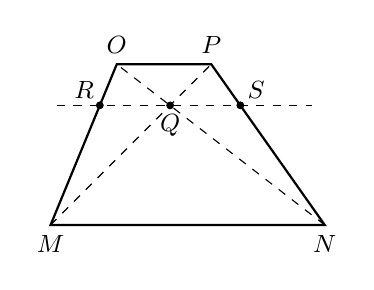
\begin{tikzpicture}[scale=1.2,font=\small]
\usetikzlibrary{calc}


\begin{scope}
\coordinate (m) at (0,0);
\coordinate (n) at (2.9,0);
\coordinate (o) at (0.7,1.7);
\coordinate (p) at (1.7,1.7);


\draw[thick] (m) node[below] {$M$} -- (n) node[below] {$N$} -- (p) node[above] {$P$} -- (o) node[above] {$O$} -- cycle;

\end{scope}


\coordinate (q) at (intersection of m--p and n--o);

\path (q) -- +(-180:1.2) coordinate (r1);
\path (q) -- +(0:1.5) coordinate (r2);

\coordinate (r) at (intersection of r1--r2 and m--o);
\coordinate (s) at (intersection of r1--r2 and n--p);

\draw[dashed] (m) -- (p);
\draw[dashed] (n) -- (o);

\draw[dashed] (r1) -- (r2);

\draw[fill] (r) circle (1pt) node[shift={(-.2,.2)}] {$R$};
\draw[fill] (s) circle (1pt) node[shift={(.2,.2)}] {$S$};
\draw[fill] (q) circle (1pt) node[shift={(0,-.25)}] {$Q$};

\end{tikzpicture}

	\caption{Esercizio~\ref{ese:6.90}}\label{fig:ese6.90}
\end{figure}

\begin{esercizio}
\label{ese:6.91}
Considerate la figura~\ref{fig:ese6.91}. \`E sufficiente sapere che $VW=2CW$ per stabilire il rapporto di similitudine tra $ABC$ e $CTU$? Se $Area(ABC) = 54$ rispetto al metro quadrato, quanto è l'area di $CTU$? Completate: <<Il rapporto tra le due parti in cui $ABC$ rimane diviso dal segmento $TU$ è \ldots{}>>.
\end{esercizio}

\begin{figure}[!htb]
	\centering% (c) 2014 Daniele Masini - d.masini.it@gmail.com
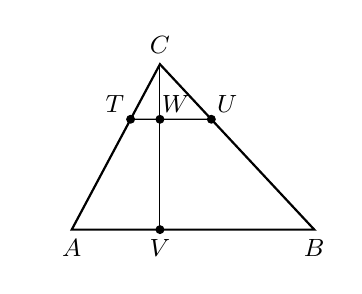
\begin{tikzpicture}[scale=1.4,font=\small]
\usetikzlibrary{calc}


\begin{scope}
\coordinate (c) at (0.8,1.5);
\coordinate (a) at (0,0);
\coordinate (b) at (2.2,0);

\draw (c) -- ($(a)!(c)!(b)$) coordinate (v);
\coordinate (w) at ($(c)!0.333!(v)$);

\path (w) -- +(-180:1.2) coordinate (r1);
\path (w) -- +(0:1.5) coordinate (r2);

\coordinate (t) at (intersection of r1--r2 and c--a);
\coordinate (u) at (intersection of r1--r2 and c--b);

\draw (t) -- (u);

\draw[thick] (a) node[below] {$A$} -- (b) node[below] {$B$} -- (c) node[above] {$C$} -- cycle;


\draw[fill] (t) circle (1pt) node[shift={(-.2,.2)}] {$T$};
\draw[fill] (u) circle (1pt) node[shift={(.2,.2)}] {$U$};
\draw[fill] (v) circle (1pt) node[below] {$V$};
\draw[fill] (w) circle (1pt) node[shift={(.2,.2)}] {$W$};

\end{scope}


\end{tikzpicture}

	\caption{Esercizio~\ref{ese:6.91}}\label{fig:ese6.91}
\end{figure}

\begin{esercizio}
\label{ese:6.92}
A che distanza dal vertice $A$ di un triangolo deve essere posto un punto $P$ sul lato $AB$ di 12~cm, in modo che la parallela condotta da $P$ al lato $BC$ determini un triangolo $APR$ che sia i $9/16$ del trapezio $PRCB$?
\end{esercizio}

\begin{esercizio}
\label{ese:6.93}
Nel triangolo rettangolo $ABC$, rettangolo in $C$, il cateto $AC$ è $3/4$ del cateto $BC$. Da un punto $D$ dell'ipotenusa si traccino le parallele al cateti. Il perimetro del rettangolo che si viene a formare è $11/6$ del cateto $BC$. Individua il rapporto di ciascuno dei lati del rettangolo con il cateto $BC$. [R.~$33/42$, $44/21$]
\end{esercizio}

\begin{esercizio}
\label{ese:6.94}
Dal punto medio $M$ dell'ipotenusa $BC$ di un triangolo rettangolo $ABC$, traccia la perpendicolare all'ipotenusa che incontra il cateto $AB$ in $D$. Determina il rapporto tra le aree dei triangoli $DMB$ e $ABC$.
\end{esercizio}

\begin{esercizio}
\label{ese:6.95}
In una circonferenza di centro $O$ e raggio di misura 30~cm, è inscritto un triangolo $ABC$ isoscele su base $BC$ con la base che è i $2/3$ della relativa altezza. Calcolare le misure dei lati di tale triangolo e il perimetro del triangolo $BCD$, essendo $D$ la proiezione ortogonale di $C$ sulla tangente in $B$ alla circonferenza. (Per rispondere alla seconda domanda tracciare l'altezza del triangolo $ABC$ relativa ad $AC$ e osservare la similitudine dei triangoli \ldots{}).
\end{esercizio}

\end{multicols}

\begin{esercizio}[Olimpiadi della Matematica - Gara di II livello, febbraio 2012]
\label{ese:6.96}
Sia $ABC$ un triangolo acutangolo; sia $O$ il suo circocentro e siano $P$ e $Q$ i punti (diversi da $A$) in cui rispettivamente l'altezza uscente dal vertice $A$ e il prolungamento di $AO$ incontrano la circonferenza circoscritta ad $ABC$. Dimostrare che
\begin{enumeratea}
\item gli angoli $B\widehat{A}P$ e $Q\widehat{A}C$ sono congruenti;
\item i triangoli $BCP$ e $CBQ$ sono congruenti;
\item detti $M$ e $N$ i punti medi di $AB$ e $AC$, l'area del quadrilatero $ABPC$ vale quattro volte l'area del quadrilatero $AMON$.
\end{enumeratea}
\end{esercizio}

\begin{esercizio}[Olimpiadi della Matematica - gara di II livello, febbraio 2006]
\label{ese:6.97}
Sia $ABC$ un triangolo e sia $A'$ il simmetrico di $A$ rispetto a $BC$; sia poi $DAA'$ simile ad $ABC$ e sia $D$ il simmetrico di $D$ rispetto ad $AA'$. Sapendo che il prodotto delle aree dei quadrilateri $ABA'C$ e $ADA'D'$ è 16, la misura di $AA'$ è
\begin{enumeratea}
\item 1;
\item $2\sqrt[4]{2}$;
\item 2;
\item $2\sqrt{2}$;
\item non è univocamente determinata dai dati.
\end{enumeratea}
(Nota: la similitudine tra $DAA'$ e $ABC$ va intesa in modo ordinato: $DA : AB = AA':BC=A'D:CA$)
\end{esercizio}

\begin{esercizio}[Olimpiadi della Matematica - gara di II livello, febbraio 2007]
\label{ese:6.98}
In un triangolo isoscele $ABC$, con $AC = BC \neq AB$, si fissi un punto $P$ sulla base $AB$. Quante posizioni può assumere, nel piano, un punto $Q$ se vogliamo che i punti $A$, $P$ e $Q$, presi in ordine qualsiasi, siano i vertici di un triangolo simile ad $ABC$?
\begin{multicols}{5}
\begin{enumeratea}
\item 0;
\item 2;
\item 3;
\item 4;
\item 5.
\end{enumeratea}
\end{multicols}
\end{esercizio}
 
\subsubsection*{\thechapter.8 - Proprietà delle secanti e delle tangenti}

\begin{esercizio}
\label{ese:6.99}
Nella figura~\ref{fig:ese6.99}, applicando il teorema delle corde, individua tutte le possibili relazioni di proporzionalità tra i segmenti.
\end{esercizio}

\begin{figure}[!htb]
	\centering% Copyright (c) 2015 Daniele Masini - d.masini.it@gmail.com

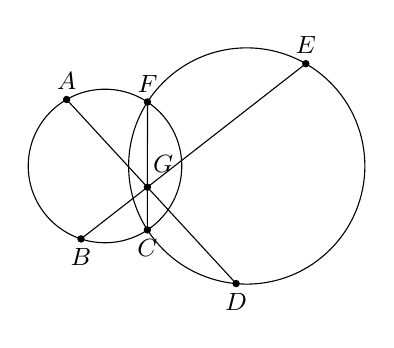
\begin{tikzpicture}[scale=.75,font=\small]
\usetikzlibrary{calc,intersections}

\begin{scope}
\pgfmathsetmacro{\raggioa}{1.3}
\pgfmathsetmacro{\raggiob}{2}
\coordinate (oa) at (0,0);
\coordinate (ob) at (2.4,0);

\draw[name path=Circle1] (oa) circle (\raggioa);

\draw[name path=Circle2] (ob) circle (\raggiob);

\path [name intersections={of=Circle1 and Circle2}] ;
\draw[fill] (intersection-1) coordinate (f) circle (1.5pt) node[above] {$F$};
\draw[fill] (intersection-2) coordinate (c) circle (1.5pt) node[below] {$C$};

\coordinate (g) at ($(f)!0.666!(c)$);

\path (ob) -- +(60:{\raggiob}) coordinate (e);

\path [name path=rettaeb] (e) -- ($(e)!1.5!(g)$);
\path [name intersections={of=Circle1 and rettaeb}] ;
\draw[fill] (intersection-2) coordinate (b) circle (1.5pt) node[below] {$B$};
\draw[fill] (e) circle (1.5pt) node[above] {$E$};

\path (oa) -- +(120:{\raggioa}) coordinate (a);
\path [name path=rettaag] (a) -- ($(a)!2.5!(g)$);
\path [name intersections={of=Circle2 and rettaag}] ;
\draw[fill] (intersection-2) coordinate (d) circle (1.5pt) node[below] {$D$};
\draw[fill] (a) circle (1.5pt) node[above] {$A$};

\draw[fill] (g) circle (1.5pt) node[shift={(0.2,0.3)}] {$G$};

\draw (a)--(d);
\draw (e)--(b);
\draw (f)--(c);

\end{scope}

\end{tikzpicture}

	\caption{Esercizio~\ref{ese:6.99}}\label{fig:ese6.99}
\end{figure}

\begin{esercizio}
\label{ese:6.100}
Individua tutte le possibili relazioni di proporzionalità tra i segmenti della figura~\ref{fig:ese6.100}, applicando il teorema delle corde.
\end{esercizio}

\begin{figure}[!htb]
	\centering% (c) 2014 Daniele Masini - d.masini.it@gmail.com
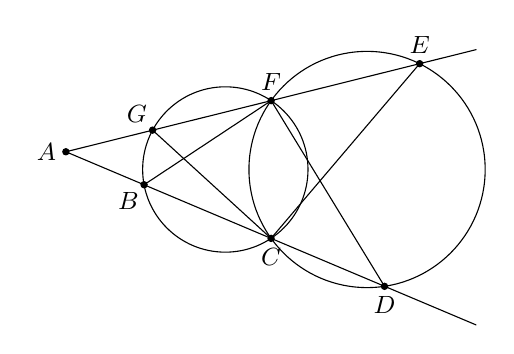
\begin{tikzpicture}[scale=.75,font=\small]
\usetikzlibrary{calc,intersections}

\begin{scope}
\pgfmathsetmacro{\raggioa}{1.4}
\pgfmathsetmacro{\raggiob}{2}
\coordinate (oa) at (0,0);
\coordinate (ob) at (2.4,0);

\draw[name path=Circle1] (oa) circle (\raggioa);

\draw[name path=Circle2] (ob) circle (\raggiob);

\path [name intersections={of=Circle1 and Circle2}] ;
\draw[fill] (intersection-1) coordinate (f) circle (1.5pt) node[above] {$F$};
\draw[fill] (intersection-2) coordinate (c) circle (1.5pt) node[below] {$C$};

\coordinate (a) at (-2.7,0.3);

\path [name path=rettaae] (a) -- ($(a)!2!(f)$) coordinate (ae);
\path [name path=rettaad] (a) -- ($(a)!2!(c)$) coordinate (ad);


\path [name intersections={of=Circle1 and rettaae}] ;
\draw[fill] (intersection-2) coordinate (g) circle (1.5pt) node[shift={(-.2,.2)}] {$G$};
\path [name intersections={of=Circle2 and rettaae}] ;
\draw[fill] (intersection-1) coordinate (e) circle (1.5pt) node[above] {$E$};

\path [name intersections={of=Circle1 and rettaad}] ;
\draw[fill] (intersection-1) coordinate (b) circle (1.5pt) node[shift={(-.2,-.2)}] {$B$};
\path [name intersections={of=Circle2 and rettaad}] ;
\draw[fill] (intersection-2) coordinate (d) circle (1.5pt) node[below] {$D$};

\draw[fill] (a) circle (1.5pt) node[left] {$A$};

\draw (a)--(ae);
\draw (a)--(ad);
\draw (g)--(c);
\draw (b)--(f);
\draw (f)--(d);
\draw (c)--(e);

\end{scope}

\end{tikzpicture}


	\caption{Esercizio~\ref{ese:6.100}}\label{fig:ese6.100}
\end{figure}

\begin{esercizio}
\label{ese:6.101}
Siano $A$, $B$, $C$ e $D$ quattro punti di una circonferenza, presi nell'ordine indicato. Sia $E$ il punto di intersezione di $AC$ con $BD$. Dimostra che i triangoli $AEB$ e $DEC$ sono simili.
\end{esercizio}

\begin{esercizio}
\label{ese:6.102}
Dato un angolo acuto di vertice $A$ e lati le semirette $r$ e $s$, traccia un punto $M$ interno all'angolo. Da $M$ traccia la perpendicolare a $r$ che la incontra in $B$ e che taglia $s$ in $C$. Sempre da $M$ traccia la perpendicolare a $s$ che la incontra in $D$ e che taglia $r$ in $E$. Dimostra che i punti $B$, $D$, $C$ ed $E$ stanno su una stessa circonferenza. 
\end{esercizio}

\begin{esercizio}
\label{ese:6.103}
Sia $ABC$ un triangolo circoscritto a una circonferenza $\gamma$, sia $D$ il punto di tangenza del lato $AB$ ed $E$ il punto di tangenza del lato $AC$. Sia $F$ il punto di intersezione della secante $BE$ con la circonferenza. Dimostra che i triangoli $DBF$ e $BDE$ sono simili. (Applica il teorema della secante e della tangente).
\end{esercizio}

\begin{esercizio}
\label{ese:6.104}
In una circonferenza di centro $O$, due corde $AB$ e $CD$ si incontrano in un punto $P$. Sapendo che $\overline{PO}=2$~cm e che $\overline{AP}\cdot \overline{BP}=\np{14,02}$~cm\textsuperscript{2}, calcola il raggio della circonferenza. [R.~\np{4,24}~cm]
\end{esercizio}

\begin{esercizio}
\label{ese:6.105}
Una corda $AB$ di una circonferenza misura 3~cm. Dal punto medio $M$ della corda passa un'altra corda della stessa circonferenza, tale che $MD=CM+2$~cm. Determina la lunghezza della corda $CD$. [R.~\np{3,6}~cm]
\end{esercizio}

\begin{esercizio}[Olimpiadi della Matematica - gara di II livello, febbraio 2007]
\label{ese:6.106}
\`E data una circonferenza di diametro $AB$ e centro $O$. Sia $C$ un punto della circonferenza (diverso da $A$ e da $B$) e si tracci la retta $r$ per $O$ parallela ad $AC$. Sia $D$ l'intersezione di $r$ con la circonferenza dalla parte opposta di $C$ rispetto ad $AB$. Dimostrare che $DO$ è bisettrice dell'angolo $C\widehat{D}B$ e che il triangolo $CDB$ è simile al triangolo $AOD$. (La similitudine è dimostrabile in due modi \ldots{}).
\end{esercizio}

\subsubsection*{\thechapter.9 - La sezione aurea}

\begin{esercizio}
\label{ese:6.107}
Assegnato un segmento $AB$, costruite il rettangolo avente per lati la sezione aurea del segmento e la diagonale del quadrato avente $AB$ come lato.
\end{esercizio}

\begin{esercizio}
\label{ese:6.108}
Un rettangolo $ABCD$ ha il lato $AD$ che è la sezione aurea del lato $AB$; verificate che, dopo aver costruito all'interno del rettangolo il quadrato $AEFD$ di lato $AD$ ($E$ su $AB$ e $F$ su $DC$), il segmento $EB$ è sezione aurea di $AD$. Costruite ora entro $EBCF$ il quadrato di lato $EB$ e verificate che il rettangolo che rimane ha il lato minore che è sezione aurea del lato maggiore. Potete affermare che tutti i rettangoli che via via si possono costruire sono tra loro simili? Calcolate il valore esatto del rapporto aureo, supponendo unitaria la misura del lato $AB$ del rettangolo aureo descritto nell'esercizio precedente: $\dfrac{AB}{BC}=\dfrac{1}{\ldots{}}\simeq \np{1,}\ldots{}$
\end{esercizio}

Il rettangolo dell'esercizio~\ref{ese:6.108} viene chiamato \emph{rettangolo aureo} in quanto risulterebbe, tra gli infiniti rettangoli che si possono disegnare, quello che dà la maggiore ``soddisfazione visiva''; il rapporto tra $AB$ e $AD$ viene chiamato \emph{numero aureo}. 
Negli oggetti quotidiani possiamo trovare alcuni esempi di rettangolo aureo: le schede telefoniche, le carte di credito e bancomat, le SIM dei cellulari, sono tutti rettangoli aurei.
Ritroviamo il rettangolo aureo anche in opere architettoniche e pittoriche: il grande scultore greco Fidia, collaborando alla costruzione del Partenone, seguì il rapporto aureo; il viso della Gioconda di Leonardo da Vinci può essere racchiuso in un rettangolo aureo; nella ``Parade'', opera del pittore francese Seurat, vari punti delimitano rettangoli aurei; ``Place de la Concorde'', un'astrazione lineare di Piet Mondrian, è costituita da rettangoli aurei che si sovrappongono.

\begin{figure*}[!htb]
	\centering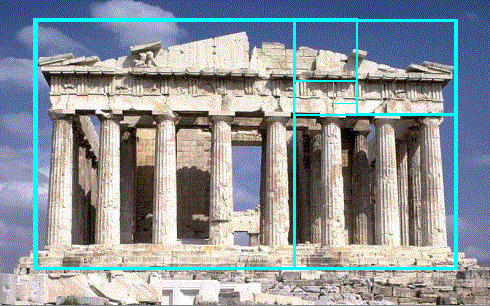
\includegraphics[width=0.57\textwidth]{partenone.png}\qquad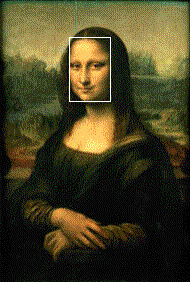
\includegraphics[width=0.24\textwidth]{monna_lisa.png}
\end{figure*}

\begin{esercizio}
\label{ese:6.109}
Il numero aureo è solitamente indicato con la lettera greca $\phi$; esso è un numero irrazionale con alcune caratteristiche: se considerate l'approssimazione $\phi=\np{1,618033989}\ldots{}$ e determinate $\phi^2$ e $1/\phi$ potete notare che \ldots\ldots{}
\end{esercizio}

\begin{esercizio}
\label{ese:6.110}
Dimostrate che nel triangolo isoscele $ABC$ di base $BC$ e con angolo al vertice di $108\grado$, il lato è la sezione aurea della base. (Tracciate una semiretta di origine $A$ che spezzi l'angolo in due parti di cui una doppia dell'altra \ldots{}).
\end{esercizio}

\begin{esercizio}
\label{ese:6.111}
Dimostrate che il lato del pentagono regolare è la sezione aurea della diagonale.
\end{esercizio}

\noindent\begin{minipage}{0.7\textwidth}\parindent15pt
\begin{esercizio}
\label{ese:6.112}
Dal quadrato $ABCD$ nella figura a fianco, costruiamo un rettangolo aureo.
\begin{enumerate*}
\item Congiungete i punti medi $E$ ed $F$ rispettivamente dei lati $AB$ e $CD$.
\item Con centro in $E$ descrivete l'arco di circonferenza di raggio $EC$ che interseca in $G$ il prolungamento di $AB$ (dalla parte di $B$).
\item Da $G$ innalzate la perpendicolare ad $AG$ che interseca in $H$ il prolungamento del lato $DC$.
\end{enumerate*}
Il rettangolo $AGHD$ è un rettangolo aureo. Infatti l'arco di circonferenza passa anche per il vertice $D$; $H$ è un punto esterno da cui esce la secante \ldots{} e il segmento di tangente \ldots\ldots{}
Si ha la proporzione \ldots\ldots\ldots\ldots{} da cui si deduce la suddetta conclusione.
\end{esercizio}
\end{minipage}\hfil
\begin{minipage}{0.3\textwidth}
	\centering% (c) 2014 Daniele Masini - d.masini.it@gmail.com
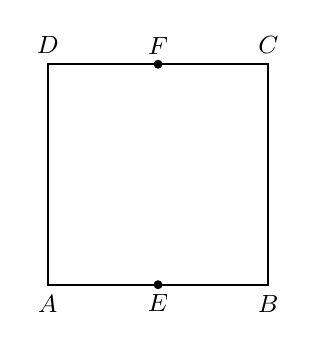
\begin{tikzpicture}[scale=1.4,font=\small]
\usetikzlibrary{calc}


\begin{scope}

\draw[thick] (0,0) node[below] {$A$} -- (2,0) node[below] {$B$} -- (2,2) node[above] {$C$} -- (0,2) node[above] {$D$} -- cycle;

\draw[fill] (1,0) circle (1pt) node[below] {$E$};
\draw[fill] (1,2) circle (1pt) node[above] {$F$};

\end{scope}

\end{tikzpicture}



\end{minipage}
